\documentclass{standalone}
\usepackage{tikz}
\usepackage{ctex,siunitx}
\setCJKmainfont{Noto Serif CJK SC}
\usepackage{tkz-euclide}
\usepackage{amsmath}
\usetikzlibrary{patterns, calc}
\usetikzlibrary {decorations.pathmorphing, decorations.pathreplacing, decorations.shapes,}
\begin{document}
\small
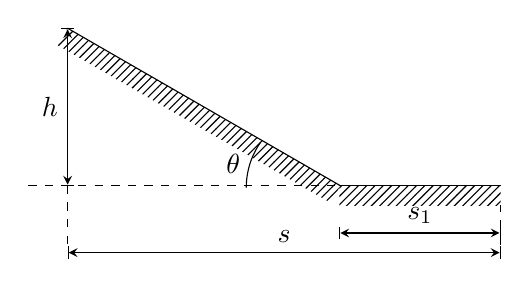
\begin{tikzpicture}[>=stealth,scale=1]
  \fill [pattern = north east lines, rotate=-30] (0,-.25) rectangle (4,0);
  \draw [rotate=-30](0,0)--(4,0);
  \fill [pattern = north east lines] (3.45,-2) rectangle (5.5,-2-.25);
  \draw (3.45,-2)--(5.5,-2);
  \draw[|<->|] (3.45,-2.6)--(5.5,-2.6)node[midway,above]{$s_1$};
  \draw[|<->|] (0,-2.85)--(5.5,-2.85)node[midway,above]{$s$};
  \draw[|<->|] (0,0)--node[midway,left]{$h$}(0,-2);
  \draw[dashed] (-0.5,-2)--(3.45,-2);
  \draw[dashed] (0,-2)--(0,-2.75);
  \draw[dashed] (5.5,-2.75)--(5.5,-2.25);
  \draw  (3.45-1,-2+.55)   arc (145:180:1)node[midway,left] {$\theta$};
\end{tikzpicture}
\end{document}